\newpage
\section{Implementierung PWA}
Schritte der Implementierung
\begin{enumerate}
	\item Einrichten der Entwicklungsumgebung
	\item Initialisierung des Projekts
	\item Installation der Pakete
\end{enumerate}

\subsection{Einrichten der Projektumgebung}
Für die Entwicklung der PWA wird die Entwicklungsumgebung Webstorm von JetBrains gewählt, da sie die viele Routineaufgaben selbstständig beziehungsweise mit geringem Aufwand ausführt.

Wie für die Entwicklung der meisten modernen Webanwendungen ist die Installation der Node.js Laufzeitumgebung notwendig. Mit dem integrierten Paketmanager npm lassen sich Bibliotheken leicht zum Projekt hinzufügen.
Um die Angular Anwendung automatisiert zu erstellen, ist zuerst die Installation des Angular \acf{cli} erforderlich. Mit dem Konsolenbefehl \texttt{npm install -g @angular/cli} wird npm aufgefordert, die neuste Version der Angular CLI global auf dem System zu installieren.


Mit dem Befehl \texttt{ng new todoapp} wird die Angular CLI (in der Konsole als \texttt{ng} abgekürzt) dazu gebracht, ein Angularprojekt inklusive nötiger Dateistrukturen zu erstellen.
\begin{wrapfigure}{r}{0.6\textwidth}
	\vspace{-10pt}
	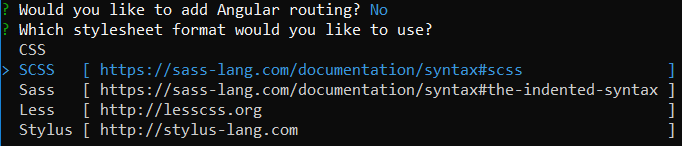
\includegraphics[width=0.58\textwidth]{img/angular_cli_css.PNG}
	\caption{Stylesheetformate beim Erstellen der Angularanwendung}
	\label{fig:stylesheet_formate_cli}
	\vspace{-10pt}
\end{wrapfigure}
Die CLI bietet dem Nutzer einige Optionen bei der Erstellung an, die jedoch in diesem Projekt nicht zwangsläufig benötigt werden, so kann beispielsweise ein Routing oder Unittesting eingerichtet werden.
Außerdem unterstützt die CLI verschiedene Stylesheetformate (siehe Abbildung \ref{fig:stylesheet_formate_cli}). Das ist für Entwickler*innen sehr praktisch, wenn sie einen dieser CSS-Dialekte beherschen. Die Arbeit mit Variablen in Stylesheets bevorzugt wird, werden in diesem Projekt SCSS Dateien verwendet.


\subsection{Angular}

Im Folgenden werden die einzelnen Komponenten der Angular-Anwendung erläutert. Es wird explizit darauf hingewiesen, dass \textbf{Quellcode-Ausschnitte teilweise stark gekürzt worden sind}, um die Lesbarkeit zu erhöhen.

\subsubsection{Klasse TodoItem zur Datenspeicherung}

Die Komponenten tauschen untereinander Daten aus. Damit diese einer einheitlichen Struktur folgen, wird eine Klasse \texttt{TodoItem} erstellt, die einen Todo-Eintrag repräsentiert. Objekte dieser Klasse können jetzt einfach zwischen Komponenten ausgetauscht und modifiziert werden.

\begin{listing}[h]
	\inputminted{TypeScript}{sourcecode/pwa_todoitem_klasse.js}
	\caption{TodoItem-Klasse zur Datenspeicherung (gekürzt)}
	\label{sourcecode:todoitem_klasse}
\end{listing}

Wie im Ausschnitt \ref{sourcecode:todoitem_klasse} zu sehen, hat ein Todo-Element eine Aufgabenbeschreibung (Zeile 2), zwei boolsche Werte, die speichern, ob das Element als wichtig oder abgeschlossen markiert worden ist (Zeile 4 und 5) und eine eindeutige ID (Zeile 2). Die ID hilft später ein bestimmtes Todo-Element zu modifizieren.

\subsubsection{\texttt{todoService} für die Datenverwaltung}
Alle Todo-Einträge sollen persistent auf dem Gerät gespeichert werden. Dafür wird ein Angular-Service erstellt: der \texttt{todoService}. Er ist für die \acf{crud} Operationen zuständig.

\begin{listing}[h]
	\inputminted{TypeScript}{sourcecode/pwa_todo_service.ts}
	\caption{Klasse \texttt{TodoService} (gekürzt)}
	\label{sourcecode:pwa_todo_service}
\end{listing}

In Ausschnitt \ref{sourcecode:pwa_todo_service} sind die Kernfunktionen des Services abgebildet. Der Service speichert ein Array von \texttt{TodoItem}-Objekten. Wenn der*die Nutzer*in ein Element hinzufügt, erstellt der Service ein neues Datenobjekt und speichert dieses im Array und dem Browserspeicher (Zeilen 16-18). Die Funktionsweise der übrigen CRUD-Operationen ist analog dazu.

Mit \texttt{localStorage} (Zeilen 8-14) kann auf den Key-Value-Store des Browsers zugegriffen werden. Beim Speichern werden die Todo-Elemente als JSON-Objekt im Store abgelegt und analog dazu geladen.

\subsubsection{Dateistruktur und Komponenten der Angularanwendung}
Nach dem im Vorangegangenen beschrieben worden ist, wie das Projekt erstellt worden ist, wird im Folgenden detaillierter auf das erstellte Angular-Projekt eingegangen. Angular, welches stark komponentenorientiert aufgebaut ist, zeigt sich auch in seiner Dateistruktur stark komponentenbezogen. In Abbildung \ref{fig:pwa_dateistruktur} sind die wichtigsten Dateien in einem Diagramm dargestellt.

\begin{figure}[H]
	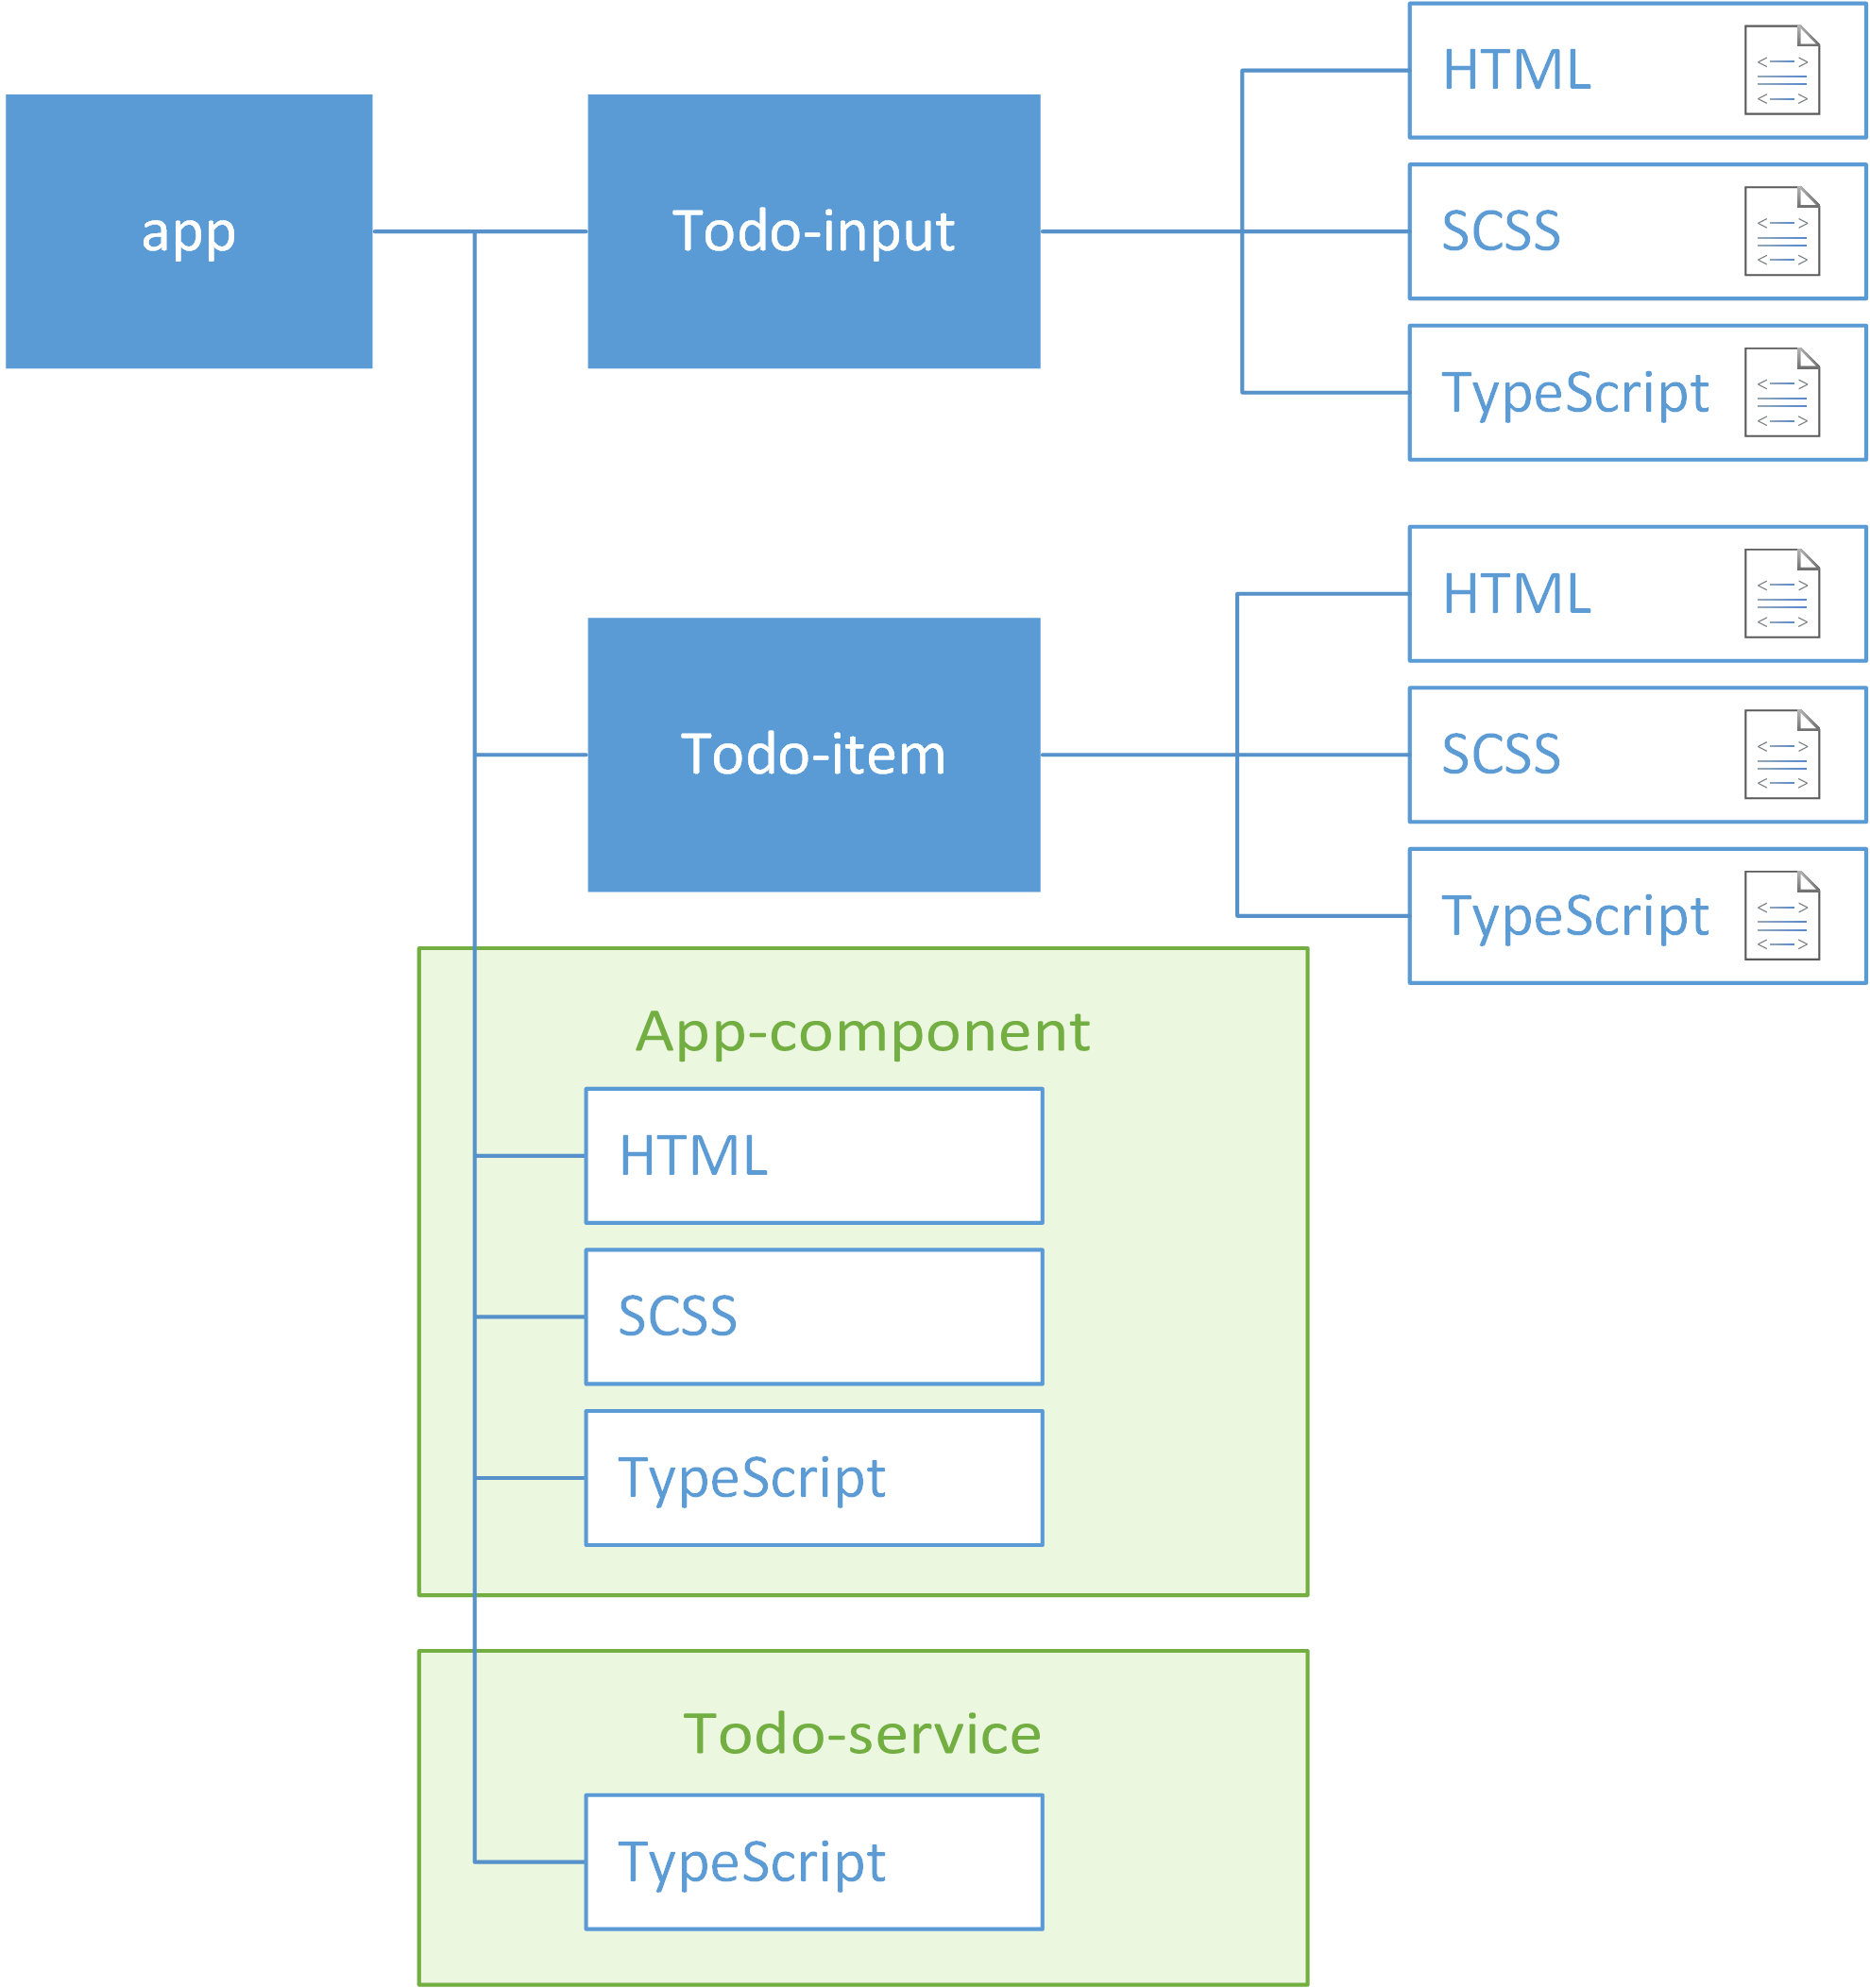
\includegraphics[width=0.6\textwidth]{img/pwa_dateistruktur.png}
	\centering
	\caption{Dateistruktur der Angularanwendung}
	\label{fig:pwa_dateistruktur}
\end{figure}

\begin{description}
	\item[Stammkomponente] Zunächst befinden sich im \texttt{app} Verzeichnis eine HTML-, eine Stylesheet- und eine TypeScript-Datei der \texttt{app-component}: die Stammkomponente. Sie dient als Container (siehe Begrifflichkeiten in Kapitel \ref{chap:grundlagen}) um die Todo-Elemente und das Inputfeld (siehe Ausschnitt \ref{sourcecode:pwa_app_component_html}, Zeile 5).
	
	\begin{listing}[h]
		\inputminted{text}{sourcecode/pwa_app_component.html}
		\caption{HTML Template der \texttt{app-component} (gekürzt)}
		\label{sourcecode:pwa_app_component_html}
	\end{listing}

	Ausschnitt \ref{sourcecode:pwa_app_component_html}, Zeilen 1-3, zeigt, wie die Daten aus dem \texttt{todoService} in HTML-Code dargestellt werden. Wie in einer For-Schleife, wird jedes item des \texttt{todoService} einer neu erstellten \texttt{todo-item}-Komponente übergeben.
	Angular wird das HTML-Template automatisch neu rendern, wenn sich die items im \texttt{todoService} ändern.
	
	
	
	
	\item[Todo-item] 
	Das \texttt{todo-item} ist ein einzelnes Elemente der Todo-Liste. Es enthält einen Button zum priorisieren, eine Checkbox zum abhaken des Elements, eine Textbox und einen Button zum Löschen (siehe Abbildung \ref{fig:pwa_todo_item_screenshot}).
	
	\begin{figure}[h]
		
\includegraphics[width=0.6\textwidth]{img/pwa_todo_item.PNG}
		\centering
		\caption{Gerender \texttt{todo-item}}
		\label{fig:pwa_todo_item_screenshot}
	\end{figure}
	
	
	Es ist sinnvoll jedes Listenelement in einer mehrfach instanziierten Komponente zu repräsentieren. Dies kapselt die Daten des Listenelements und die Kommunikation mit dem \texttt{todoService} von anderen Listenelementen ab. Wie bereits erwähnt bekommt jede \texttt{todo-item}-Komponente genau ein Objekt der Klasse \texttt{TodoItem} übergeben.
	
	\begin{listing}[h]
		\inputminted{text}{sourcecode/pwa_todo_item.html}
		\caption{HTML Template der \texttt{todo-item} (gekürzt)}
		\label{sourcecode:pwa_todo_item_html}
	\end{listing}

	Ausschnitt \ref{sourcecode:pwa_todo_item_html} zeigt das HTML-Template des \texttt{todo-item}. Die ersten drei Input-Elemente werden durch \texttt{[(ngModel)]} mit einer Property des \texttt{TodoItem}s verknüpft, welche in der \texttt{todo-item}-Komponente gespeicht wird. Dies bewirkt folgenden Mechanismus: Wird das Input-Element verändert, ändert sich auch das gespeicherte \texttt{TodoItem}. Würde das \texttt{TodoItem} im Code modifiziert, ändert aktualisiert sich das Input-Element entsprechend.
	
	Um modifizierte Daten auch in der Datenquelle zu speichern, wird das modifizierte \texttt{TodoItem} bei jeder Änderung dem \texttt{todoService} übergeben.
	
\end{description}

\begin{figure}[h]
	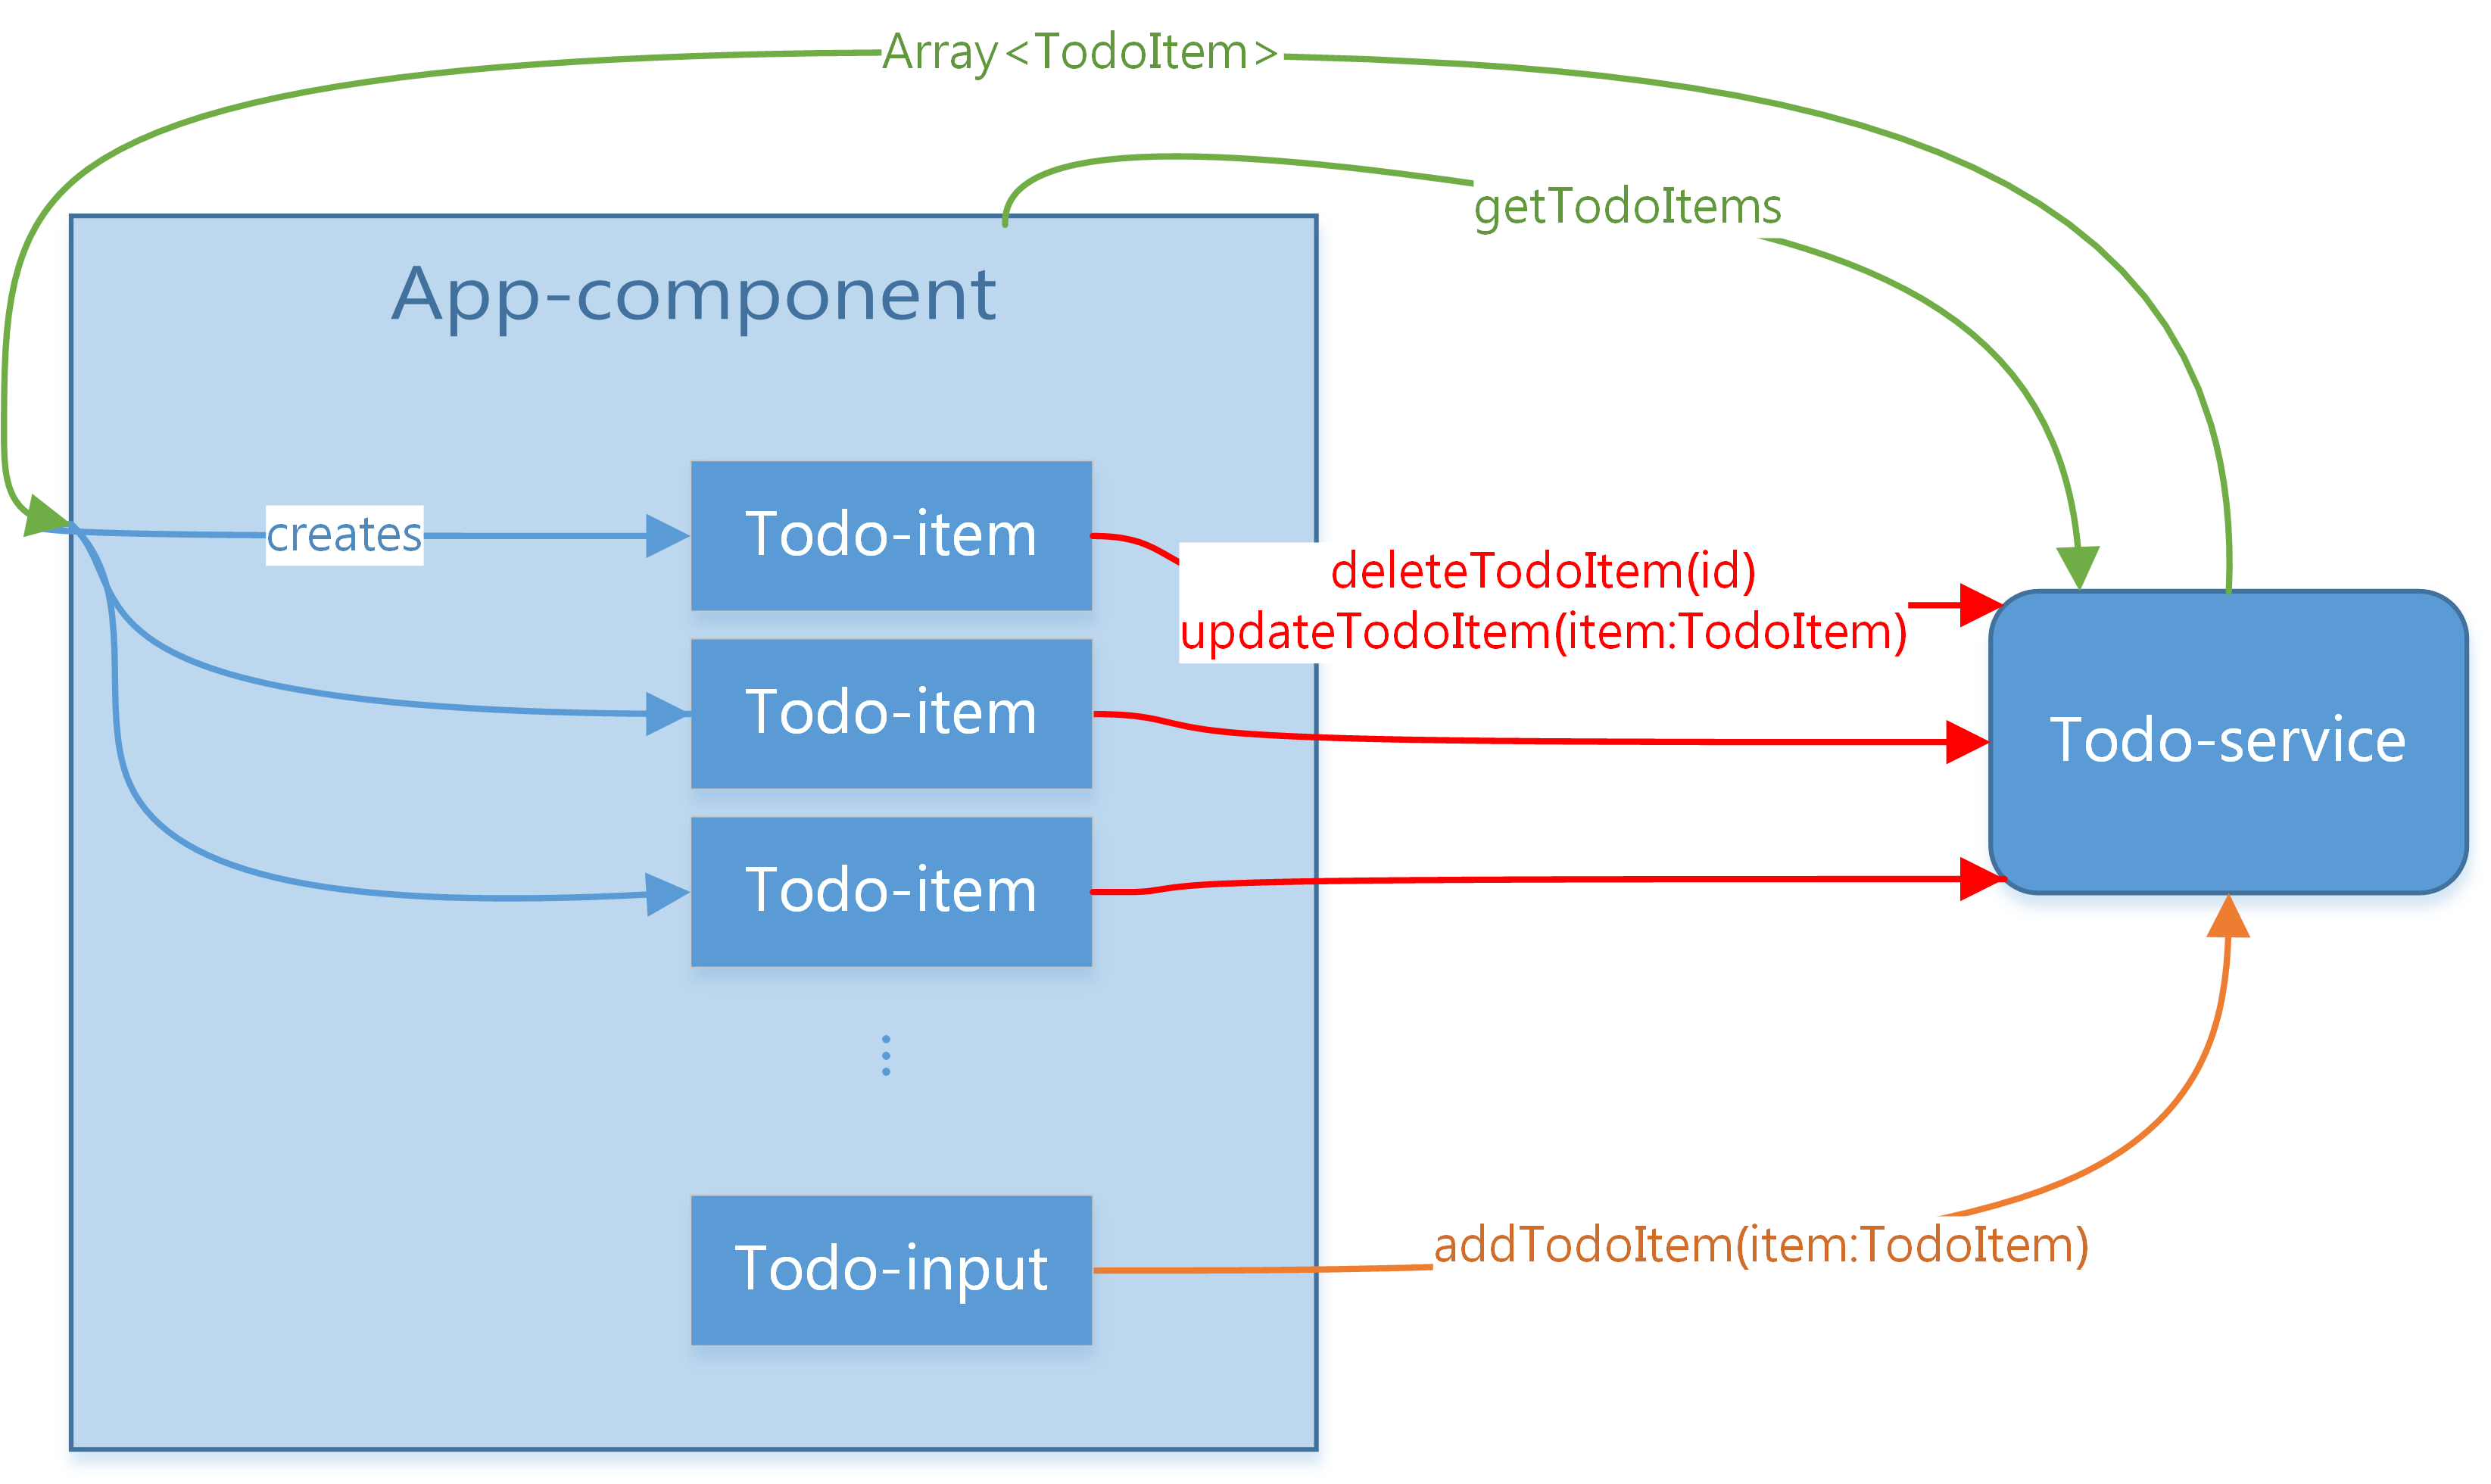
\includegraphics[width=\textwidth]{img/pwa_components.png}
	\centering
	\caption{Interaktion des Todo-service mit den Komponenten}
	\label{fig:pwa_todo_service}
\end{figure}

\begin{figure}[h]
	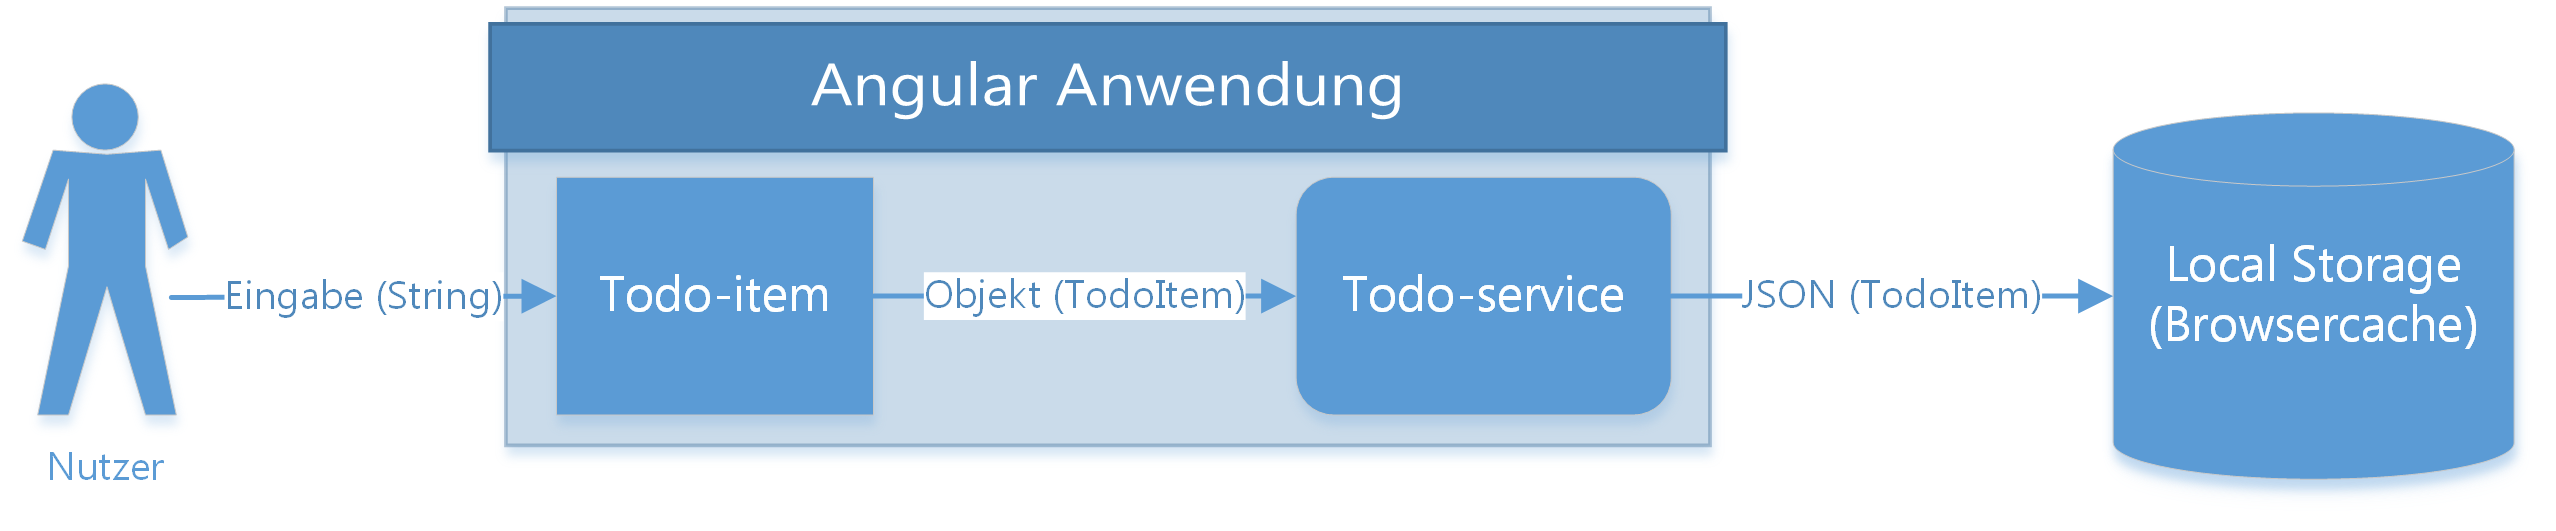
\includegraphics[width=\textwidth]{img/pwa_datenfluss_eingabe.png}
	\centering
	\caption{Datenfluss bei Änderung eines Todo Eintrages}
	\label{fig:pwa_datenfluss_eingabe}
\end{figure}

\begin{figure}[h]
	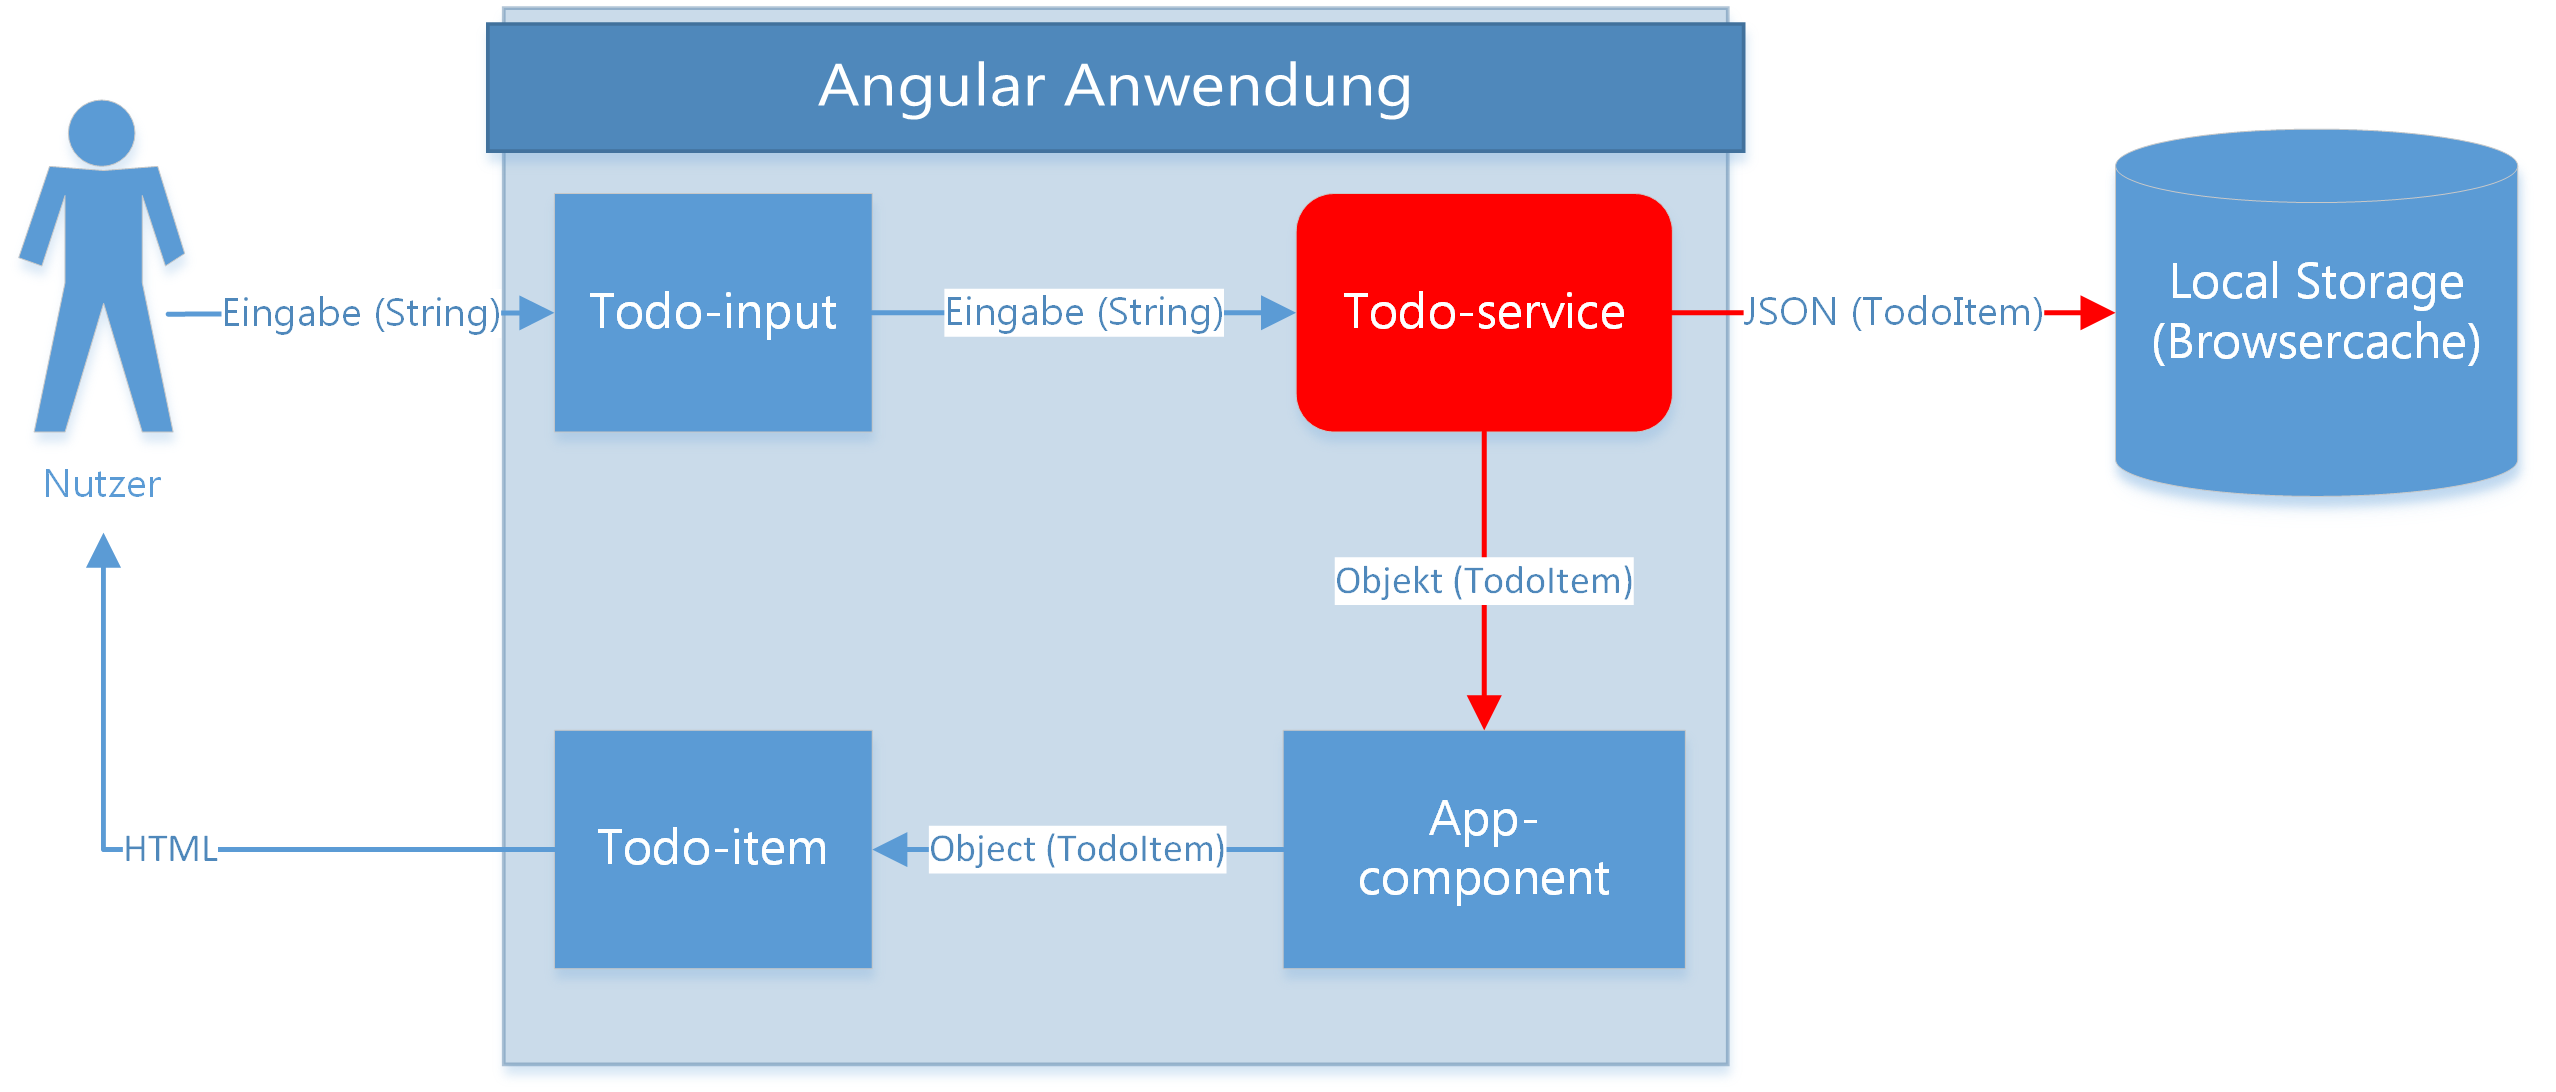
\includegraphics[width=\textwidth]{img/pwa_datenfluss_erstellen.png}
	\centering
	\caption{Datenfluss bei Erstellung eines Todo Eintrages}
	\label{fig:pwa_datenfluss_erstellen}
\end{figure}


\subsection{Hosting der App}
Damit die PWA als solche installiert werden kann muss sie bestimmte Kriterien erfüllen (siehe Kapitel \ref{chap:grundlagen}). Darunter ist die Notwendigkeit der Bereitstellung über HTTPS. Dies gestaltet sich in der Praxis als schwierig, da der Angular Entwicklungsserver zwar auf HTTPS konfiguriert werden kann, jedoch selbstsignierte SSL Zertifikate nicht aktzeptiert werden: Die PWA kann nicht installiert werden. Für die Entwicklung ist das natürlich problematisch, so dass eine Lösung für dieses Problem gefunden werden muss.

Googles stellt eine schnelle und elegante Lösung zum Hosten einer Webanwendung bereit: Firebase. Über die Firebase Console, eine Webanwendung zur Verwaltung von Firebase Projekten, kann innerhalb weniger Minuten ein Projekt inklusive Hosting erstellt werden.

Das dem Firebase CLI können automatisiert Konfigurationsdateien für das Firebase Hosting angelegt werden. Die Schritte dazu sind ebenfalls trivial:
\begin{enumerate}
	\item \textbf{Anmeldung: \\}
	      Das CLI muss mit einem Google-Konto verknüpft werden. Dazu beim Login über das CLI ein Browserfenster mit einem Google-Login Dialog.
	\item \textbf{Initialisierung: \\}
	      Die Initialisierung über das CLI legt unter anderem eine JSON-Datei zur Konfiguration des Deployments an. Hier werden Dateipfade, wie beispielsweise die Start-URL oder Dateien die deployed werden sollen, gespeichert.
	\item \textbf{Deployment: \\}
	      Über die Angular CLI wird ein sogenannter Production-Build erstellt. Dies ist eine gepackte Version der Webanwendung für den Produktivbetrieb.
	      Anschließend kann die gepackte Anwendung mit \texttt{firebase deploy} auf einem von Googles Servern bereitgestellt werden.
\end{enumerate}

Die Anwendung läuft jetzt mit einer validen HTTPS-Verbindung und kann von Nutzern installiert werden.

Das Hosting mit Firebase löst gleichzeitig ein weitere Problem: das Testen der Anwendung auf einem Smartphone. Die von Firebase bereitgestellte URL kann jetzt einfach im mobilen Chromebrowser aufgerufen und installiert werden.

\subsection{Installation der Anwendung}
\textbf{Smartphones:}\\
Nach dem Aufrufen der URL mit dem mobilen Browser, erscheint eine Meldung zum Installieren der PWA (siehe \ref{fig:dialog_install_pwa_mobile}).

\begin{figure}[h]
	
\includegraphics[scale=0.5]{img/pwa_add_to_homescreen.png}
	\centering
	\caption{Browserdialog zum Installieren der PWA als Windows Desktop App}
	\label{fig:dialog_install_pwa_mobile}
\end{figure}

\textbf{Desktop:}
\begin{wrapfigure}{r}{0.5\textwidth}
	\vspace{-10pt}
	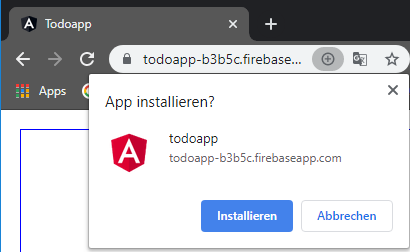
\includegraphics[width=0.48\textwidth]{img/add_to_desktop_2.PNG}
	\caption{Browserdialog zum Installieren der PWA als Desktop App}
	\label{fig:dialog_install_pwa_mobile}
	\vspace{-10pt}
\end{wrapfigure}
In der Suchleiste von Chrome, kann der Nutzer die PWA als Desktopanwendung installieren (siehe \ref{fig:dialog_install_pwa_mobile}).
\begin{wrapfigure}{L}{0.5\textwidth}
	\vspace{-10pt}
	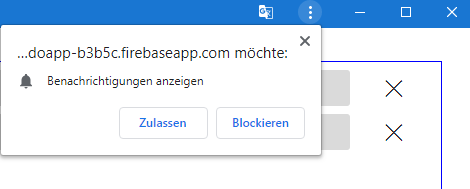
\includegraphics[width=0.48\textwidth]{img/berechtigungen_zulassen.PNG}
	\centering
	\caption{Dialog für Benachrichtigungen}
	\label{fig:pwa_benachrichtigungen_zulassen}
	\vspace{-10pt}
\end{wrapfigure}
Damit dem Nutzer Benachrichtigungen tatsächlich angezeigt werden, muss er beim erhalten der ersten Nachricht die Benachrichtigungen über einen Dialog aktivieren (siehe \ref{fig:pwa_benachrichtigungen_zulassen}).

\subsection{Prüfung der Browserunterstützung}
Für Webanwendungen ist es üblich, diese mit verschiedenen Browsern zu testen. Um das Kriterium der Plattformabhängigkeit detailliert evaluieren zu können, erscheint es ebenfalls sinnvoll, die Installation der PWA sowohl auf dem Desktop, als auch auf Android und iOS Smartphones zu testen.

\textbf{Anmerkung:}\\
Zum Testen der Datenpersistenz werden Todo-Einträge angelegt und anschließend der Browser neugestartet.
Alle Browser werden mit Standardeinstellungen ausgeführt. Es werden keine Browsercaches, Cookies oder ähnliches manuell gelöscht.

\textbf{Desktop:}

\begin{table}[H]
	\centering
	\begin{tabularx}{\textwidth}{|l||C|C|C|C|}
		\hline
		Browser              & Anwendung lauffähig & Persistente Daten & PWA installierbar & Benachrichtigungen \\
		\hline
		Chrome 78 (64-bit)   & Ja                  & Ja                & Ja                & Ja                 \\
		Firefox 70 (64-bit)  & Ja                  & Ja                & Nein              & Ja                 \\
		Microsoft Edge 41    & Ja                  & Ja                & Nein              & Nein               \\
		Internet Explorer 11 & Ja                  & Ja                & Nein              & Nein               \\
		Safari 13            & Ja                  & Ja                & Nein              & Nein               \\
		\hline
	\end{tabularx}
	\caption{Browserunterstützung Desktop} \label{tab:browser_desktop}
\end{table}

\textbf{Anmerkung:}\\
Microsoft Edge und Internet Explorer zeigen den Button zum Priorisieren nicht an. Dieser enthält ein Unicodezeichen eines Sterns.

Microsoft Edge möchte die Zustimmung des Nutzers, um Benachrichtigungen anzuzeigen, zeigt jedoch anschließend keine Benachrichtigungen an. Internet Explorer wirft den JavaScript Fehler \texttt{'Notification' is undefined}, Notifications sind nicht implementiert.

\textbf{Smartphone:}

\begin{table}[H]
	\centering
	\begin{tabularx}{\textwidth}{|l||C|C|C|C|}
		\hline
		Browser           & Anwendung lauffähig & Persistenz & PWA installierbar & Benachrichtigungen \\
		\hline
		\multicolumn{5}{|c|}{Android}                                                                 \\
		\hline
		Chrome 78         & Ja                  & Ja         & Ja                & Ja                 \\
		Firefox 68        & Ja                  & Ja         & Ja                & Ja                 \\
		Microsoft Edge 41 & Ja                  & Ja         & Nein              & Ja                 \\
		Opera 54          & Ja                  & Ja         & Nein              & Ja                 \\
		\hline
		\multicolumn{5}{|c|}{iOS}                                                                     \\
		\hline
		Chrome            & Ja                  & Ja         & Nein              & Nein               \\
		Safari 13         & Ja                  & Ja         & Nein              & Nein               \\
		\hline
	\end{tabularx}
	\caption{Browserunterstützung Smartphones} \label{tab:browser_smartphones}
\end{table}

\textbf{Anmerkung:}\\
Verweigert der Nutzer die Benachrichtigungen einer Webseite, ist es meist umständlich die Berechtigung für Benachrichtigungen einer Website zurückzusetzen. Beim Browser Opera muss der Nutzer dann beispielsweise durch fünf Menüs nacheinander navigieren, um die deaktivierten Benachrichtigungen wieder zu aktivieren.

\subsection{Update der Anwendung}

Um das Updateverhalten zu evaluieren, ist es interessant, den Updateprozess einer Webanwendung beziehungsweise PWA zu betrachten. Um Änderungen an die Nutzer zu verteilen, muss ein Entwickler*in einen neuen Production Build auf dem Server bereitstellen. Im Falle diese Projekts werden Änderungen unter Nutzung der Firebase CLI auf den Server übertragen.
In der Praxis werden die Änderungen in der installierte PWA nicht sofort sichtbar, wohingegen die Webanwendung beim nächsten Refresh der Seite aktualisiert wird. Dies hängt mit dem Caching der Ressourcen der PWA zusammen. Der Service Worker lädt cachbare Dateien entweder beim Start oder nachträglich während die PWA läuft in den lokalen Cache des Geräts.

Um dieses Verhalten zu Testen wurde ein Update mit einer auffälligen Hintergrundfarbe auf dem Server bereitgestellt. In der Desktop-PWA war die Änderung erst nach einem Systemneustart zu sehen, wohingegen sich die PWA unter Android nach einigen Stunden automatisch aktualisierte.



\subsection{Hinzufügen der Manifestdatei}
https://medium.com/poka-techblog/turn-your-angular-app-into-a-pwa-in-4-easy-steps-543510a9b626

\subsection{Desktop}


Der verwendete Entwicklungsbrowser Chromium bietet keine Möglichkeit die PWA als Desktopanwendung zu installieren.



